%%%%%%%%%%%%%%%%%%%%%%%%%%%%%%%%%%%%%%%%%%%%%%%%%%%%%%%%%%%%%%%%%%%
%                                                                 %
%  GEANT manual in LaTeX form                              %
%                                                                 %
%  Michel Goossens (for translation into LaTeX)                   %
%  Version 1.00                                                   %
%  Last Mod. Jan 24 1991  1300   MG + IB                          %
%                                                                 %
%%%%%%%%%%%%%%%%%%%%%%%%%%%%%%%%%%%%%%%%%%%%%%%%%%%%%%%%%%%%%%%%%%%
\Origin{R.Brun, P.Zanarini}
\Revision{S.Giani}
\Documentation{P.Zanarini, S.Giani, F.Carminati}                   
\Submitted {01.10.83}                   \Revised{13.12.93}
\Version{Geant 3.16}                    \Routid{DRAW300}
\Makehead{Handling View banks}
\section{The view banks}
The basic detector drawing routines (\Rind{GDRAW}, \Rind{GDRAWC}, 
\Rind{GDRAWX}) scan the data structure {\tt JVOLUM} repeatedly to
extract position and dimension information on the volumes. This can
be a rather lengthy process even on fast computer. 
Hidden line removal drawing requires
an auxiliary data structure and the 
relative visibility of all the volumes has to be analysed. With complicated 
detectors the time spent in this process can be substantial, depending 
on the drawing options chosen and on the speed of the machine on which 
the program is run. In order to alleviate this problem the graphic
{\it banks} and the associated routines have been developed.

The interpretation
of the structure (for instance scanning of the volumes' data structure 
to convert the 3D geometry structure into a set 
of 2D lines, visibility analysis, surface creation or
light processing) is thus separate
from the drawing itself. In this way, the interpretation is performed 
only once and all the 2D information is stored in view banks (data 
structure {\tt JDRAW} {\tt [DRAW399]}). These views can then be displayed
quickly, having only to draw the 2D vectors or the fill
areas previously stored. 

For a detector with more than 100 different volumes, for example, 
this costs only a few thousand words of memory for 
each drawing stored.

If the drawing routines are called while a view bank, identified by
a positive integer, is open (\Rind{GDOPEN})
only interpretation will be made,
no output will be generated until the bank is closed (\Rind{GDCLOS}).
When a view bank has been closed it cannot be modified, but
it can be displayed as many times as wanted (\Rind{GDSHOW}) or deleted
(\Rind{GDELET}).

Once a drawing (detectors, tracks or hits) is in a view bank, it is 
possible to scan it in detail via the {\tt LENS} or {\tt ZOOM} interactive
commands (only available with {\tt X11}). For more information see
the {\tt [XINT]} section.

\Shubr{GDOPEN}{(IVIEW)}

\begin{DLtt}{MMMMMMMM}
\item[IVIEW] ({\tt INTEGER}) view bank number ({\tt IVIEW>0}).
\end{DLtt}

Opens a {\it view bank}, used to store 2D graphics information
coming from the interpretation of 3D structures (but also 2D annotation).
All subsequent calls to the drawing routines will fill the
view bank {\tt IVIEW}, without generating any output.
\Shubr{GDCLOS}{}
Closes the current opened view bank. Once a view bank has been closed
no more drawing can be added to it. A call to \Rind{GDCLOS} also restores the
screen.

\Shubr{GDSHOW}{(IVIEW)}

\begin{DLtt}{MMMMMMMM}
\item[IVIEW] ({\tt INTEGER}) view bank number ({\tt IVIEW>0}).
\end{DLtt}

Displays view bank {\tt IVIEW}. \Rind{GDSHOW} can be called either
before or after a view bank has been closed. If a view bank is currently
open, the content of bank {\tt IVIEW} will be added to it.

\begin{figure}[hbt]
     \centering
     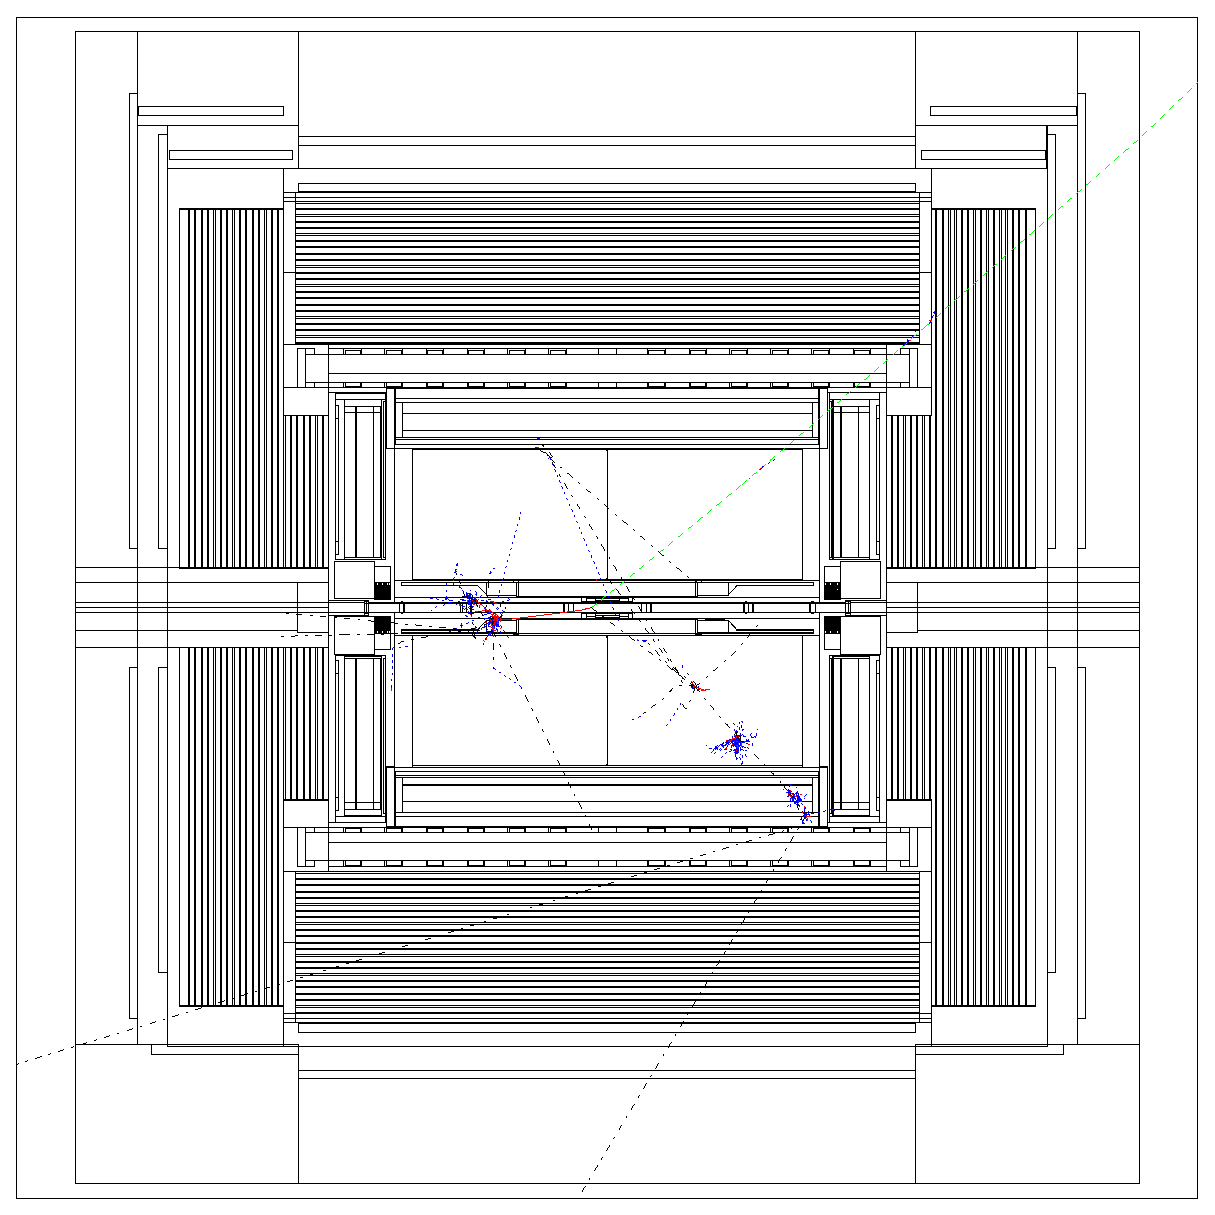
\epsfig{file=eps/draw300-1.eps,width=12.cm}
\begin{verbatim}
      CALL GDOPEN(3)
      CALL GDRAWC('ALEF',2,5.,10.,10.,0.013,0.013)
      CALL GDCLOS
      CALL GDSHOW(3)
      .
      .
      CALL GDXYZ(0)
\end{verbatim}
     \caption{Example of use of view banks}
     \label{fg:draw300-1}
\end{figure}
 
\Shubr{GDELET}{(IVIEW)}

\begin{DLtt}{MMMMMMMM}
\item[IVIEW] ({\tt INTEGER}) view bank number ({\tt IVIEW>0}).
\end{DLtt}

Deletes a view bank from memory. If called before a bank has been closed,
\Rind{GDELET} will also restore the screen mode. 

{\bf Note:} the {\tt JDRAW} data structure has a top level bank which 
contains one word for each view bank in {\tt Q(JDRAW+IVIEW)}. This
word is a key which determines the status of the bank. If this key 
is 3, the bank itself is protected against deletion, and it cannot be 
deleted by \Rind{GDELET}. An example of use of view banks is shown in 
Fig.~\ref{fg:draw300-1}.
